\section{Schema ER}

	Riportiamo in Figura \ref{fig:schemaER} lo schema ER del database e in Figura \ref{fig:schemaTabelle} uno schema più ad alto livello che permette di farsi direttamente un'idea dell'organizzazione in tabelle.
	
\begin{figure}[h]
	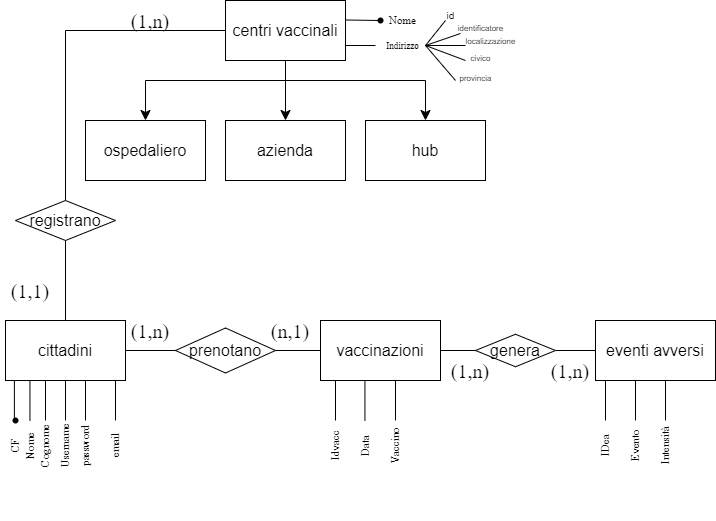
\includegraphics[width=\textwidth]{./img/ER}
	\caption{Schema ER della base di dati}
	\label{fig:schemaER}
\end{figure}

\begin{figure}[h]
	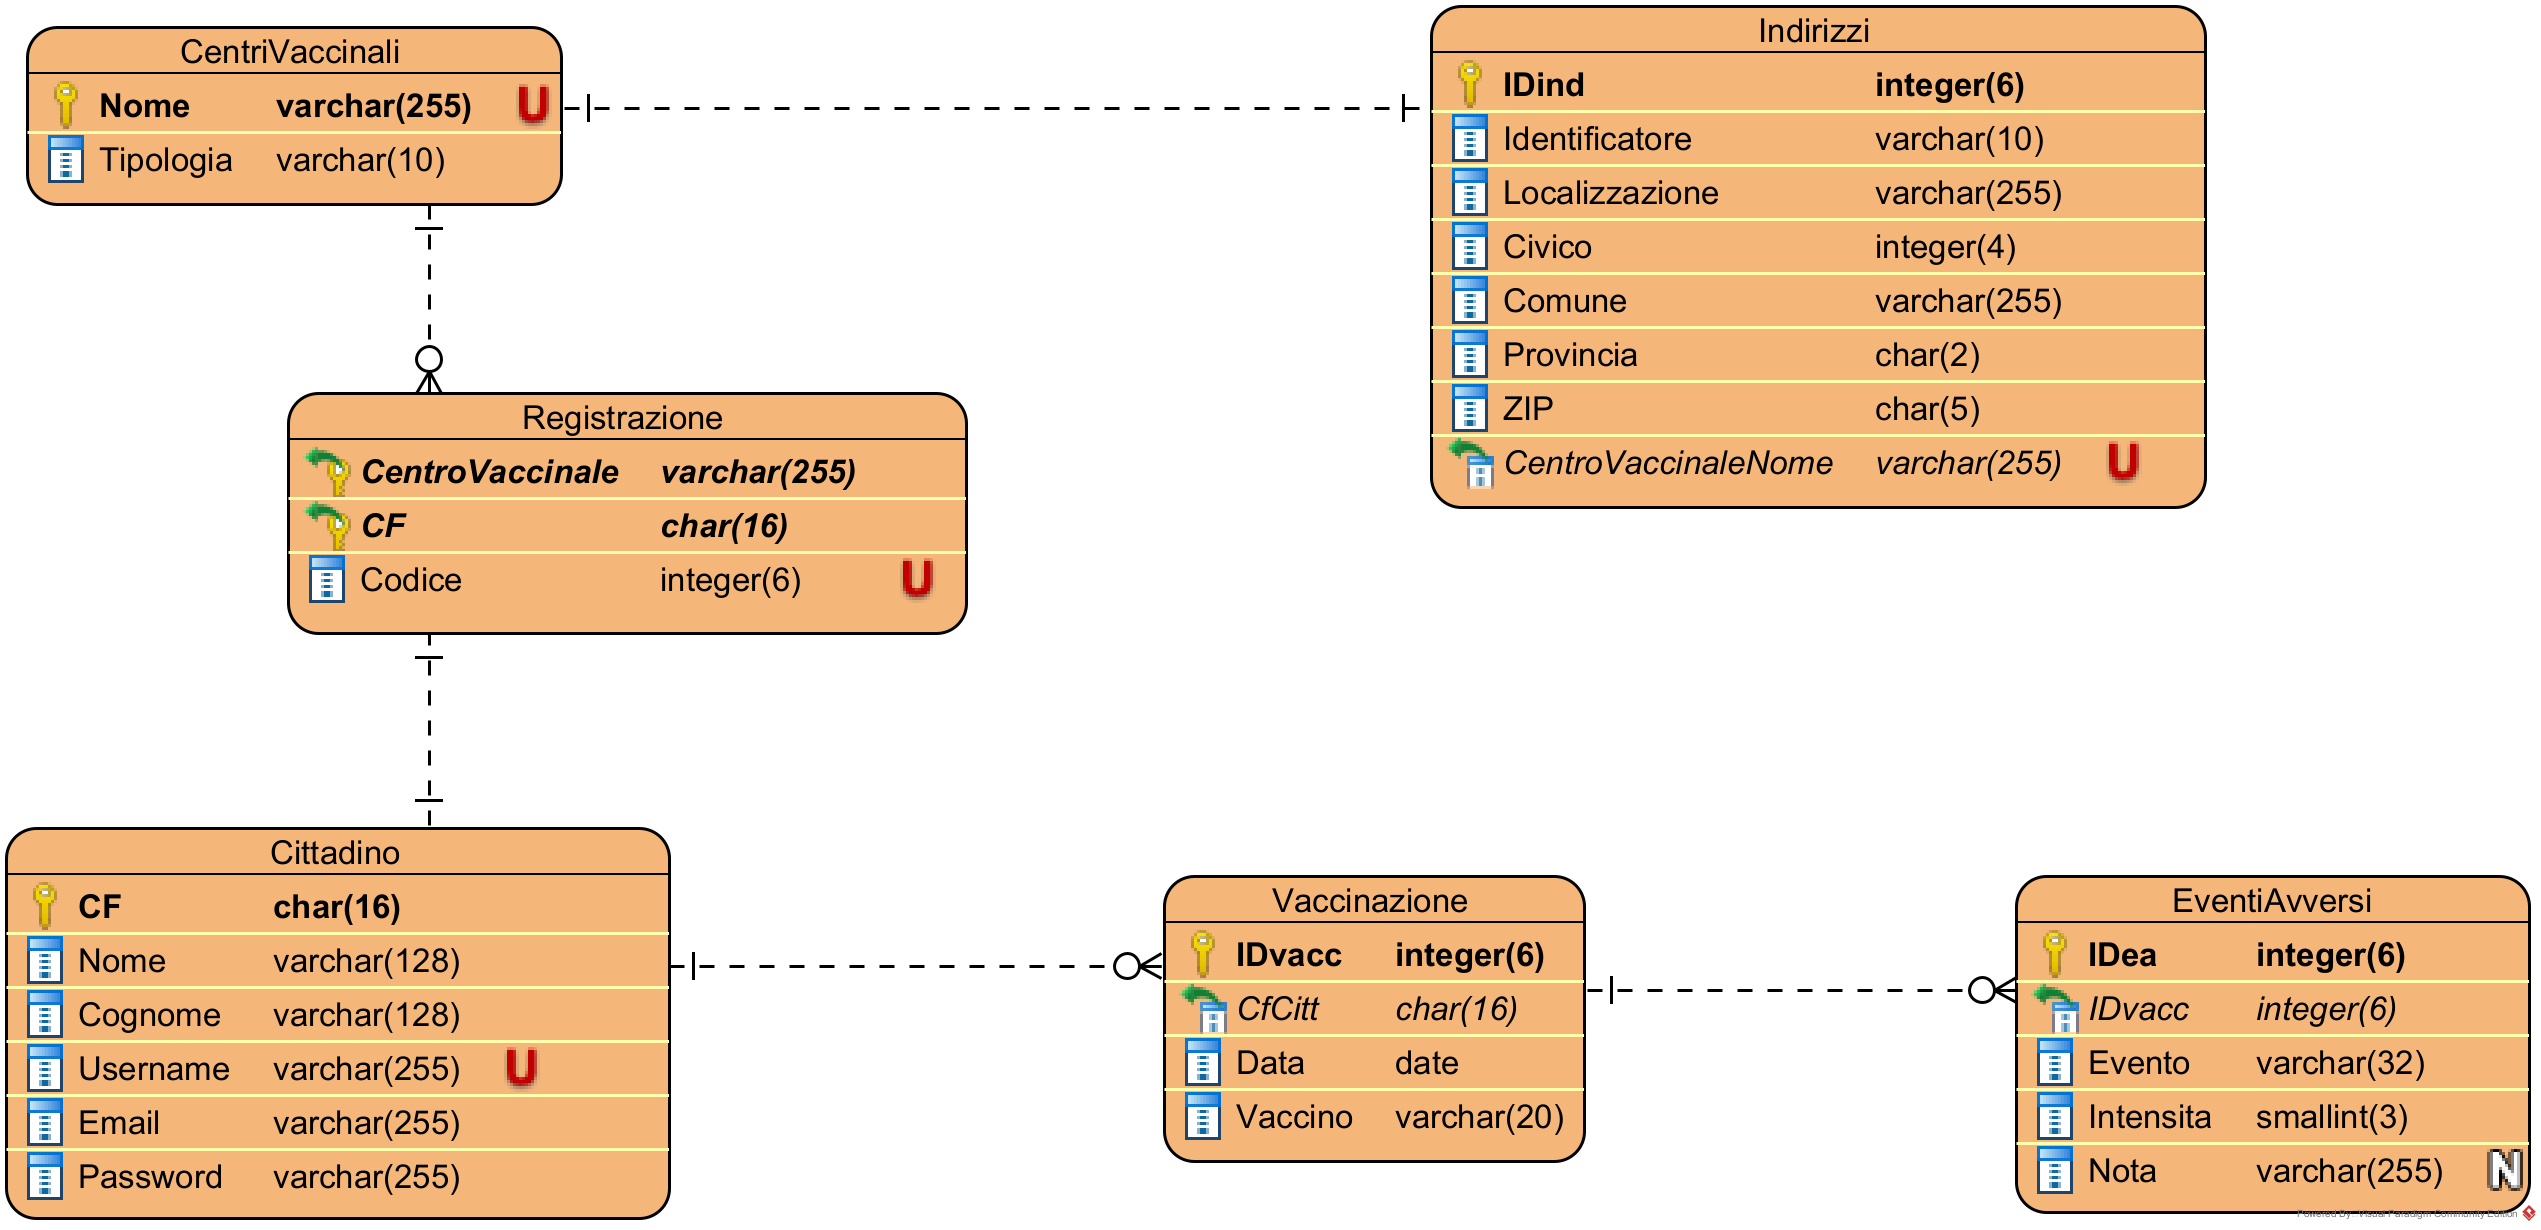
\includegraphics[width=\textwidth]{./img/CentriVaccinaliDB}
	\caption{Schema delle tabelle del database}
	\label{fig:schemaTabelle}
\end{figure}